%!TEX root = /Users/rafaeldurelli/Dropbox/Artigos Elaborados/KDM propagation_2015/sbes_2015_kdm_propagation/sbes2015_kdm_propagation.tex

\section{Evaluation}\label{sec:evaluation}

This section describes the experiment used to evaluate the effectiveness of our DI Algorithm, step [B] of our approach. Therefore, we have compared its result with an oracle in order to verify its correctness. %The second experiment is referred as ``Propagation Study'' and was planned to evaluated the correctness of the propagation given a set of refactorings. 
In addition, we have worked out one research question, as follows:
%
%Moreover, this experiment also evaluate the devised Eclipse plug-in, which was earlier described. Specifically, we investigate the following research questions:
%
\textbf{RQ$_{1}$}: Given some specific elements to be refactored, is the DI Algorithm able to identify correctly all the dependent KDM elements?

%\textbf{RQ$_{2}$}: Given a specific refactoring R, are all dependent elements identified in the oracle correctly refactored?
 
%To evaluate these questions we we carried out two steps. Firstly, we have evaluated our mining algorithm. Therefore, we have compared its result with an oracle in order to verify its correctness. Similarly, we have evaluated the correctness of a set of refactorings. Thus,  we have also compared its results to the same oracle mentioned previously.

\subsection{Goal Definiton}\label{sec:goal_definition}

We use the organization proposed by the Goal/Question/Metric (GQM) paradigm, it describes experimental goals in five parts, as follows:
%
%\begin{itemize}
%
%\item \textbf{object of study:} the object of study is our approach; 
%
%\item \textbf{purpose:} the purpose of this experiment is to evaluate the effectiveness of our mining approach; %The experiment provides insight into how much effective can be our mining approach. It is also expected that the experimental results can be used to evaluate the impact of idenfiforking the execution of mutant methods in their own threads and weakly killing them have on the performance.
%
%\item \textbf{perspective:} this experiment is run from the standpoint of a researcher;
%
%\item \textbf{quality focus:} the primary effect under investigation is the precision and recall after applying the mining algorithm; 
%
%\item  \textbf{context:} this experiment was carried out using Eclipse 4.3.2 on a 2.5 GHz Intel Core i5 with 8GB of physical memory running Mac OS X 10.9.2.
%\end{itemize}
%
(\textit{i}) \textbf{object of study:} the object of study is our approach; (\textit{ii}) \textbf{purpose:} the purpose of this experiment is to evaluate the effectiveness of our DI Algorithm, i.e., step [B] of our whole approach; (\textit{iii}) \textbf{perspective:} this experiment is run from the standpoint of a researcher; (\textit{iv}) \textbf{quality focus:} the primary effect under investigation is the precision and recall after applying the DI Algorithm; (\textit{v}) \textbf{context:} this experiment was carried out using Eclipse 4.3.2 on a 2.5 GHz Intel Core i5 with 8GB of physical memory running Mac OS X 10.9.2.

The experiment can be summarized using Wohlin et al.'s template~\cite{Wohlin} as follows: 

\textbf{Analyze} the effectiveness of our DI Algorithm

\textbf{for the purpose of} evaluation

\textbf{with respect to} precision and recall

\textbf{from the point of view of} the researcher

\textbf{in the context of} a subject program. 

%The experiment can be defined as: \textbf{Analyze} the effectiveness of our mining algorithm, \textbf{for the purpose of} evaluation, \textbf{with respect to} precision and recall, \textbf{from the point of view of} the researcher, \textbf{in the context of} a subject program. 

\subsection{Effectiveness Analysis}\label{hypothesis_formulation}	

Herein we present an effectiveness analysis aiming to determine the recall and precision of our approach. To do that, we have applied our DI Algorithm, step [B], in one system and compared the results with oracles and a manual analysis. The system we have used as case studies was LabSys, the same system used in the case study. This analysis employs the metrics Recall and Precision, which are described below:

\begin{itemize}
\item Precision is the ratio of the number of true positives retrieved to the total number of irrelevant and relevant KDM elements retrieved/propagated. It is usually expressed as a percentage, see equation 1.
\end{itemize}
%In order to accomplish our goal, we explored the formalization of our research question into hypotheses so that statistical tests can be performed. The hypotheses are shown in Table~\ref{tab:hypotheses}. There are two variables shown on each table: `P' and `R'. `P' stands for Precision which is the ratio of the number of true positives retrieved/identified to the total number of irrelevant and relevant code elements retrieved/propagated. It is usually expressed as a percentage, see equation 1. `R' denotes Recall which is the ratio of the number of true positives retrieved/propagated to the total number of relevant code elements in the source code. It is usually expressed as a percentage, see equation 2. 

%\begin{table}[h]
%\centering
%\caption{Hypotheses for the Mining Study\label{tab:hypotheses}}
%~~\\
%\begin{tabularx}{
%.46\textwidth}{|c|X|}
%There is no difference between using our tool and using an ad-hoc reuse process in terms of productivity (time) to couple sucessfully a CF with an application.
%\hline \cellcolor[gray]{\shadow} H$_0$ & \footnotesize{ There is no difference in pattern recognition before and after to apply our mining affected metaclasses algorithm into the KDM model (measured in terms of the metric precision (P) and recall (R)) which can be formalized as: 

%\textbf{H$_{0}$: $\mu_{P_{Bf}} = \mu_{P_{Af}}$ and $\mu_{R_{Bf}} = \mu_{R_{Af}}$}}
%\\
%\hline \cellcolor[gray]{\shadow} H$_1$ & \footnotesize{There is a significant difference in pattern recognition before and after to apply our mining affected metaclasses algorithm into the KDM model (measured in terms of the metric precision (P) and recall (R)) which can be formalized as: 

%\textbf{H$_{1}$: $\mu_{P_{Bf}} \neq \mu_{P_{Af}}$ and $\mu_{R_{Bf}} \neq \mu_{R_{Af}}$}}
%\\
%\hline
%\end{tabularx}
%\end{table}

%\begin{table}[h]
%\centering
%\caption{Hypotheses for the Propagation Study\label{tab:hypotheses}}
%~~\\
%\begin{tabularx}{
%.46\textwidth}{|c|X|}
%There is no difference between using our tool and using an ad-hoc reuse process in terms of productivity (time) to couple sucessfully a CF with an application.
%\hline \cellcolor[gray]{\shadow} H$_0$ & \footnotesize{ There is no difference in propagation of changes before and after to apply a refactoring into the KDM model (measured in terms of the metric precision (P) and recall (R)) which can be formalized as: 

%\textbf{H$_{0}$: $\mu_{P_{Bf}} = \mu_{P_{Af}}$ and $\mu_{R_{Bf}} = \mu_{R_{Af}}$}}
%\\
%\hline \cellcolor[gray]{\shadow} H$_1$ & \footnotesize{There is a significant difference in propagation of changes before and after to apply a refactoring into the KDM model (measured in terms of the metric precision (P) and recall (R)) which can be formalized as:  
%
%\textbf{H$_{1}$: $\mu_{P_{Bf}} \neq \mu_{P_{Af}}$ and $\mu_{R_{Bf}} \neq \mu_{R_{Af}}$}}
%\\
%\hline
%\end{tabularx}
%\end{table}

%\textbf{Null hypothesis, H$_{0}$}: There is no difference in pattern recognition before and after to apply our mining affected metaclasses algorithm into the KDM model (measured in terms of the metric precision (P) and recall (R)) which can be formalized as: 

%\textbf{H$_{0}$: $\mu_{P_{Bf}} = \mu_{P_{Af}}$ and $\mu_{R_{Bf}} = \mu_{R_{Af}}$}

%\textbf{Alternative hypothesis, H$_{1}$}: There is a significant difference in pattern recognition before and after to apply our mining affected metaclasses algorithm into the KDM model (measured in terms of the metric precision (P) and recall (R)) which can be formalized as: 

%\textbf{H$_{1}$: $\mu_{P_{Bf}} \neq \mu_{P_{Af}}$ and $\mu_{R_{Bf}} \neq \mu_{R_{Af}}$}

%\textbf{Null hypothesis, H$_{0}$}: there is no difference in propagation of changes before and after to apply a refactoring into the KDM model (measured in terms of the metric precision (P) and recall (R)) which can be formalized as: 

%\textbf{H$_{0}$: $\mu_{P_{Bf}} = \mu_{P_{Af}}$ and $\mu_{R_{Bf}} = \mu_{R_{Af}}$}

%\textbf{Alternative hypothesis, H$_{1}$}: there is a significant difference in propagation of changes before and after to apply a refactoring into the KDM model (measured in terms of the metric precision (P) and recall (R)) which can be formalized as:  

%\textbf{H$_{1}$: $\mu_{P_{Bf}} \neq \mu_{P_{Af}}$ and $\mu_{R_{Bf}} \neq \mu_{R_{Af}}$}
 


\begin{equation}
Precision=\frac{True Positives}{True Positives + False Positives}
\end{equation}

\begin{itemize}
\item Recall is the ratio of the number of true positives retrieved to the total number of relevant KDM elements in the KDM instance. It is usually expressed as a percentage, see equation 2.
\end{itemize}

\begin{equation}
Recall=\frac{True Positives}{True Positives + False Negatives}
\end{equation}

\subsection{Experiment Desing}

For our evaluation, we also used the same system described in Section~\ref{sec:case_study}, LabSys. As stated before, firstly we transformed it into a KDM instance to apply our approach by means of MoDisco. %LabSys is able to allocate time to use the classes in their respective physical spaces, treat the internal communication during laboratories reservation, such as availability reports, viability, unforeseen, acceptance of a reservation, manages the equipments of laboratories, generate reports and memos about the processes.
%
%
%LabSys  was defined using the MVC architectural pattern. It contains a total of 15 packages, 113 classes, and 1307 methods. It is composed by three layers: \texttt{model}, \texttt{view}, and \texttt{controller}. Layer \texttt{model} owns the  DTO (Data Transfer Objects) and DAOs (Data Access Objects), which is represented by \texttt{Data Package}. DTO represents domain entities such as laboratories, equipments, reservations, etc. DAO is the classes that performs the database access. Layer controller is responsible for the business rules that communicates directly with model layer. Finally, view layer is the part of the software system that performs direct interaction with the user and uses the resources of controller layer. In fact, we selected this system for our validation because its code have been devised by one of the authors of this paperdetected and analyzed manually
%
%Currently, MoDisco only generates the KDM code package, other KDM packages are extremely important to evaluate our approach. Therefore, we have manually instantiated the followings KDM packages: Structure Package, Data Package, and Conceptual Package.
%
Furthermore, to evaluate our DI Algorithm it was necessary to choose some refactoring. As a matter of fact, it is important to know its parameters once our DI Algorithm uses them to identify all affected meta-classes. Therefore, we selected four refactorings and use its parameters as starting point of our mining approach. The chosen refactorings were: \textit{Extract Class}, \textit{Extract Layer}, \textit{Move Class}, and \textit{Remove Class}. %For the refactoring \textit{Extract Class} 
%
%
%We applied each of the three refactorings to every possible location in KDM instance. It is worth to notice that all refactorings were applied completely automatically by means of our devised proof-of-concept tool. To deal with refactorings that go into infinite loops, we set three minutes timeout interval. More specifically, we applied the \textit{Extract Class} to every class that had more than 300 LOC (Line of Code); we applied the \textit{Move Class} to every class from a package to another package; we applied the \textit{Pull up Method} to every method of a class that had a superclass that was not from a library, using every such superclass as the target of the pull-up. 
%
Then after applied the DI Algorithm we counted whether all the affected meta-classes were successful identified.%, i.e., if the intended refactoring could be performed, and how many propagations were generated on the model. We also counted if our DI Algorithm was effectiveness to identify all affected metaclasses after applying a refactoring. 
We also measured both software metrics precision and recall after applying the DI Algorithm on the KDM models.


%  and on the code side after to apply the refactorings. We also measured both software quality metrics Cohesion Amongst the Methods of a Class (CAMC) and Similarity- based Class Cohesion (SCC)4 before applying the refactoring on the KDM models and after applying the refactoring on the KDM models. Notice that in this case we actually measured these metrics in the code instead of the KDM model. This was possible as our proof-of-concept tool provides support for the generating of the code after one finishes to apply the refactorings.

\subsection{Analysis of Data and Interpretation}\label{analysis_of_data}

%This section presents the experimental findings. The analysis is divided into two subsections: (1) descriptive statistics and (2) hypothesis testing.

%\subsubsection{Descriptive Statistics:} This subsection provides descriptive statistics of the experiment datas. 

Table~\ref{table:precision_recall} presents both metrics: precision and recall. The each column represents the effectiveness analysis, whose goal is to analyze the recall and precision of our mining approach. In order to calculate the precision and recall values we used an oracle as the base for the comparison. This oracle has been build based on our experience in KDM models. %Fortunately, one of the author of this paper the chosen system, LabSys, HealthWatcher v10 and PetStore 1.3.2 are available [36] with the persistence concern clearly identified.
The process of checking and calculating these metrics were very time consuming because we needed to compare the log produced by our mining approach with the xml files (KDM instance). In order to help us in the identification of the most significant precision and recall we have built a bar-plot that can be seen in Figure~\ref{fig:charPrecisionAndRecall}

\begin{table}[h]
\centering
\caption{Values of precision and recall.\label{table:precision_recall}}
{\footnotesize{}}%
\setlength{\tabcolsep}{0.0em}
{\renewcommand{\arraystretch}{0.5}
\begin{tabular}{|c|c|c|c|c|c|c|c|c|}
\cline{2-9} 
\multicolumn{1}{c|}{} & \multicolumn{8}{c|}{{\footnotesize{Efectiveness Analysis}}}\tabularnewline
\cline{2-9} 
\multicolumn{1}{c|}{} & \multicolumn{2}{c|}{{\footnotesize{Extract Class }}} & \multicolumn{2}{c|}{{\footnotesize{Extract Layer}}} & \multicolumn{2}{c|}{{\footnotesize{Move Class}}} & \multicolumn{2}{c|}{{\footnotesize{Remove Class}}}\tabularnewline
\hline 
{\footnotesize{System}} & {\footnotesize{Precision}} & {\footnotesize{Recall}} & {\footnotesize{Precision}} & {\footnotesize{Recall}} & {\footnotesize{Precision}} & {\footnotesize{Recall}} & {\footnotesize{Precision}} & {\footnotesize{Recall}}\tabularnewline
\hline 
{\footnotesize{LabSys}} & {\footnotesize{100\%}} & {\footnotesize{100\%}} & {\footnotesize{80\%}} & {\footnotesize{100\%}} & {\footnotesize{100\%}} & {\footnotesize{95.11\%}} & {\footnotesize{100\%}} & {\footnotesize{90.3\%}}\tabularnewline
\hline 
\end{tabular}}
\end{table}

\begin{figure}[h]
	\centering
	% Requires \usepackage{graphicx}
	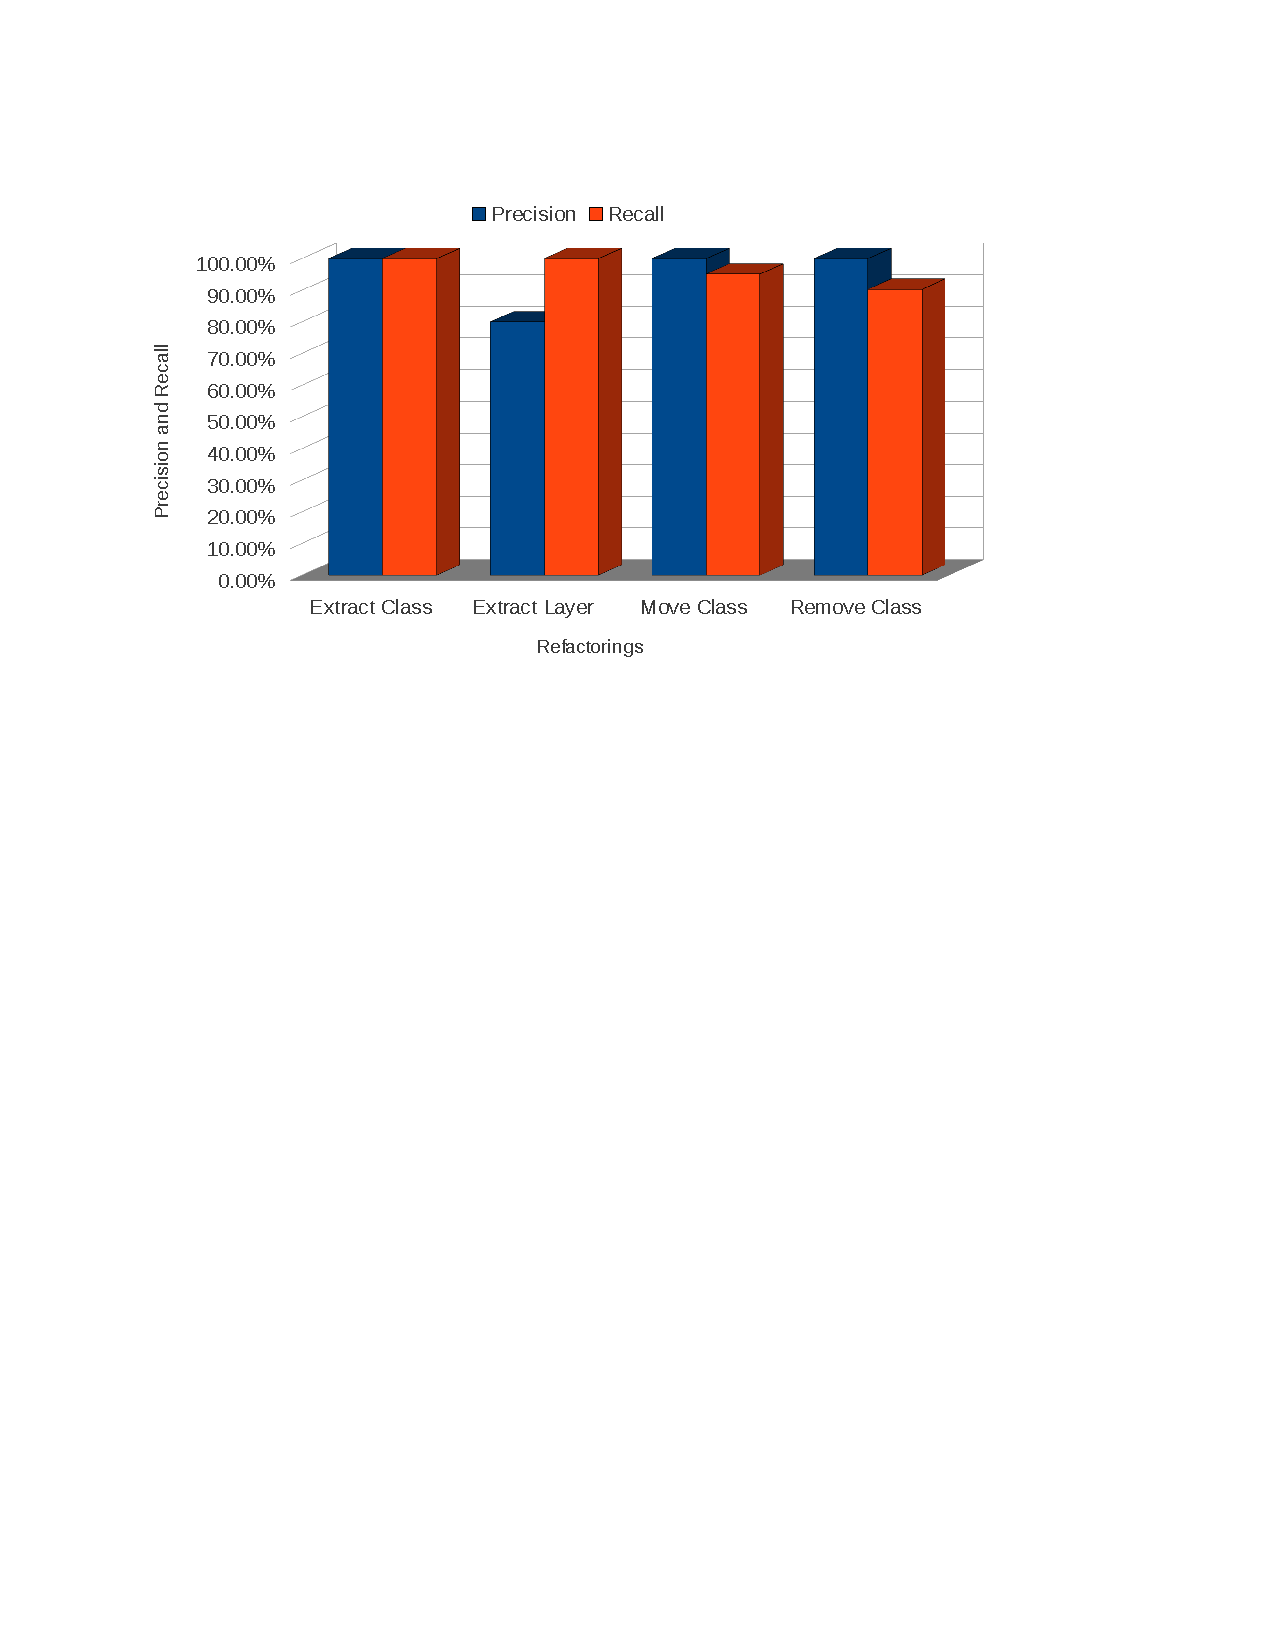
\includegraphics[scale=0.62]{figuras/barCharPrecisionAndRecall}
	\caption{Bar-plot for precision and recall of each refactoring.}
	\label{fig:charPrecisionAndRecall}
\end{figure}

Observing  both Table~\ref{table:precision_recall} and Figure~\ref{fig:charPrecisionAndRecall}, it is possible to see that for the refactoring \textit{Extract Class}'s parameters we got 100\% of precision and recall; that is there are no false negatives or positives. However, notice we got 80\% of precision for the refactoring \textit{Extract Layer}'s parameters. This happened because our mining algorithm has recognized more similar meta-classes in \textit{Extract Layer} than in \textit{Extract Class} increasing the number of false positives, as most of these meta-classes had not relation with the parameters.

Obviously, our mining algorithm failed in some cases because although some meta-classes are similar, the semantic is completely different. For example, we could have two similar instance of an specific meta-class, therefore the algorithm would identify just one. %However, it also clustered correctly the variable oafee that is a persistence field. 
As can be seen in Table~\ref{table:precision_recall} it is clear that our mining affected meta-classes algorithm helps to find meta-classes which are related with a particular refactoring but it is not foolproof. Nevertheless, empirically we can say that the algorithm add value to the whole solution.

As can be seen in our analyses, good recall and precision values were obtained using our mining affected meta-classes algorithm. Therefore, this can enable other groups to proceed researching on data mining techniques. Clearly, we cannot guarantee the same level of recall and precision but maybe it is possible to keep improving these metrics by using other data mining techniques.

\subsection{Threats to Validity}

The lack of representativeness of the subject programs may pose a threat to external validity. We argue that this is a problem that all software engineering research, since we have theory to tell us how to form a representative sample of software. %Apart from not be- ing of industrial significance, another potential threat to the external validity is that the investigated pro- grams do not differ considerably in size and complex- ity. To partially ameliorate that potential threat, the subjects were chosen to cover a broad class of applica- tions. 
Also, this experiment is intended to give some evidence of the efficiency and applicability of our implementation solely in academic settings. A threat to construct validity stems from possible faults in the implementations of the techniques. With regard to our mining techniques, we mitigated this threat by running a carefully designed test set against a complex system.